%===================================================================================
% JORNADA CIENTÍFICA ESTUDIANTIL 2013 - MATCOM, UH
%===================================================================================
% Esta plantilla ha sido diseñada para ser usada en los artículos de la
% Jornada Científica Estudiantil, MatCom 2015.
%
% Por favor, siga las instrucciones de esta plantilla y rellene en las secciones
% correspondientes.
%
% NOTA: Necesitará el archivo 'jcematcom.sty' en la misma carpeta donde esté este
%       archivo para poder utilizar esta plantila.
%===================================================================================

%===================================================================================
% PREÁMBULO
%-----------------------------------------------------------------------------------
\documentclass[a4paper,10pt,twocolumn]{article}

%===================================================================================
% Paquetes
%-----------------------------------------------------------------------------------
\usepackage{amsmath}
\usepackage{amsfonts}
\usepackage{amssymb}
\usepackage{jcematcom}
\usepackage[utf8]{inputenc}
\usepackage{listings}
\usepackage[pdftex]{hyperref}

%-----------------------------------------------------------------------------------
% Configuración
%-----------------------------------------------------------------------------------
\hypersetup{colorlinks,%
	    citecolor=black,%
	    filecolor=black,%
	    linkcolor=black,%
	    urlcolor=blue}
%===================================================================================

%===================================================================================
% Presentacion
%-----------------------------------------------------------------------------------
% Título
%-----------------------------------------------------------------------------------
\title{Proyecto de Matemática Numérica II.\\ Aplicación de la Transformada de Fourier\\ y Transformada de Wavelet en el\\ procesamiento de imágenes digitales.}

%-----------------------------------------------------------------------------------
% Autores
%-----------------------------------------------------------------------------------
\author{\\
\name Amanda Gonález Borrell \email \href{mailto:amanda.gonzalez@estudiantes.matcom.uh.c}{amanda.gonzalez@estudiantes.matcom.uh.cu}
	\\ \addr Grupo C311 \AND
\name Karla Olivera Hernández\email \href{mailto:karla.olivera@estudiantes.matcom.uh.cu}{karla.olivera@estudiantes.matcom.uh.cu}
  \\ \addr Grupo C311 \AND
\name Rodrigo García Gómez\email \href{mailto:rodrigo.garcia@estudiantes.matcom.uh.cu}{rodrigo.garcia@estudiantes.matcom.uh.cu}
  \\ \addr Grupo C312}
%-----------------------------------------------------------------------------------

%-----------------------------------------------------------------------------------
% Tutores
%-----------------------------------------------------------------------------------

%-----------------------------------------------------------------------------------
% Headings
%-----------------------------------------------------------------------------------
\jcematcomheading{2020}{1-\pageref{end}}{Amanda Gonález Borrell, Karla Olivera Hernández, Rodrigo García Gómez}

%-----------------------------------------------------------------------------------
\ShortHeadings{Ejemplo JCE}{Autores}
%===================================================================================

%===================================================================================
% DOCUMENTO
%-----------------------------------------------------------------------------------
\begin{document}

%-----------------------------------------------------------------------------------
% NO BORRAR ESTA LINEA!
%-----------------------------------------------------------------------------------
\twocolumn[
%-----------------------------------------------------------------------------------

\maketitle

%===================================================================================
% Resumen y Abstract
%-----------------------------------------------------------------------------------
\selectlanguage{spanish} % Para producir el documento en Español

%-----------------------------------------------------------------------------------
% Resumen en Español
%-----------------------------------------------------------------------------------
\begin{abstract}

 El interés de este informe se centra en proponer una solución computacional en donde se utilice en un caso La Transformada Discreta de Fourier y en otro la Transformada Discreta de Wavelet en el procesamiento de imágenes digitales, haciendo énfasis en la eliminación del ruido gaussiano en las mismas. Para ello se apoyará en las definiciones de ambas transfomadas y se utilizarán varias librerías del lenguaje de programación Python: scipy y scikit-image. Mediente el cálculo de la complejidad y los resultados de los algoritmos propuestos se establecerán comparaciones entre ambas transformadas, arrivando a concluisones de en qué escenarios es recomendado la utlización de las mismas.
	
\end{abstract}

%-----------------------------------------------------------------------------------
% English Abstract
%-----------------------------------------------------------------------------------
\vspace{0.5cm}

\begin{enabstract}

 The interest of this report is focused on proposing a computational solution where the Discrete Fourier Transform and the Discrete Wavelet Transform are used in the processing of digital images, emphasizing the elimination of Gaussian noise in them. For this, it will be supported by the definitions of both transforms and several libraries of the Python programming language will be used: scipy and scikit-image. Through the calculation of the complexity and the results of the proposed algorithms, comparisons will be established between both transforms, arriving at conclusions as to in which scenarios their use is recommended.

\end{enabstract}

%-----------------------------------------------------------------------------------
% Palabras clave
%-----------------------------------------------------------------------------------
\begin{keywords}
	transformada,
	Wavelet,
	Fourier,
	filtro.
\end{keywords}

%-----------------------------------------------------------------------------------
% Temas
%-----------------------------------------------------------------------------------

%-----------------------------------------------------------------------------------
% NO BORRAR ESTAS LINEAS!
%-----------------------------------------------------------------------------------
\vspace{0.8cm}
]
%-----------------------------------------------------------------------------------

%===================================================================================

%===================================================================================
% Introducción
%-----------------------------------------------------------------------------------
\section{Introducción}\label{sec:intro}
%-----------------------------------------------------------------------------------
 La eliminación de ruido en imágenes es un campo de investigación que ha sido de enorme interés durante las últimas décadas. Imágenes digitales se ven expuestas a ruido desde el mismo momento en que son capturadas por dispositivos digitales, ya sean cámaras, escáneres, etc. El ruido tiene diversos orígenes y ningún proceso está libre de él. Básicamente, este puede ser descrito como variaciones en los valores de los píxeles que no están asociados al objeto o fenómeno de interés por el cual se tomó la imagen. Este ruido se necesita eliminar como un paso previo al análisis y obtención de datos de ellas. Al restaurar una imagen natural, es importante que, además de eliminar el ruido, conservar sus detalles presentes, como son los bordes que delimitan a los objetos.
  
 En los últimos años se han publicado diversos métodos de suavizado de imágenes digitales, los cuales tienen como propósito eliminar pequeñas estructuras que no son de interés dentro de la imagen, las que pueden estar asociadas al ruido o a variaciones de intensidad dentro de la imagen que no necesitan ser preservadas. Este problema ha sido abordado desde varias perspectivas como en~\cite{morel05} y se continúan proponiendo nuevos algoritmos, obteniéndose cada vez mejores resultados~\cite{egiazarian09}. En la práctica, sin embargo, filtros tradicionales como el bilateral~\cite{tomasi98} continúan siendo de uso común debido a su sencillez y relativa eficacia para eliminar el ruido. Otra alternativa surge a partir de las técnicas de súper-resolución, dentro de las que han proliferado los métodos de procesamiento a nivel de subpíxel, ofreciendo una opción para aplicar también métodos de suavizado~\cite{galvez17}. Por otro lado, en~\cite{estrtada12} se propone un algoritmo novedoso para el filtrado de imágenes en niveles de gris y color. El concepto central sobre el cual se basa dicho algoritmo es una medida de correlación espacial, donde dos colores están correlacionados espacialmente si estos aparecen cercanos en la imagen con mucha frecuencia, con respecto a los otros pares de colores. En el caso discreto, dicha medida de correlación espacial se representa mediante una matriz de Adyacencia, la cual puede calcularse de manera eficiente. Otro forma de atacar este problema, fue el propuesto por~\cite{perez15}, donde se llevó a cabo el estudio de diferentes algoritmos de procesamiento de imágenes, tanto para segmentación como para eliminación de ruido Gaussiano basándose en teoría de grafos.

 El presente trabajo se centra en proponer una solución computacional en donde se utilice en un caso la Transformada Discreta de Fourier y en otro la Transformada Discreta de Wavelet en el procesamiento de imágenes, centrándose en la eliminación del ruido en las mismas. Existen varios tipos de ruidos, pero el presente trabajo se enfocará en la eliminación del ruido gaussiano, en el cual cada uno de los píxeles que componen la imagen cambia su valor de acuerdo con una distribución normal o gaussiana.

%===================================================================================

%===================================================================================
% Desarrollo
%-----------------------------------------------------------------------------------
\section{Definiciones}\label{sec:dev}
%-----------------------------------------------------------------------------------

\subsection{Transformada Discreta de Fourier}
  La \textbf{transformada discreta de Fourier} no es otra cosa que un cambio de coordenadas en $C^N$ entre dos bases que tienen un significado especial. Se define formalmente como la transformaci\'{o}n $F_N : C^N \rightarrow C^N$ que a cada vector $f \in C^N$ le hace corresponder el vector 
$\hat{f} = (\hat{f}(0),\hat{f}(1), ..., \hat{f}(N-1))$ donde 
$$\hat{f}(k) = \sum_{n = 0}^{N-1} f(n)e ^ \frac{-2i \pi kn}{N}$$
para $0 \leq n \leq N-1$. \\

 Por otra parte, otra definici\'{o}n de la que se estará haciendo referencia es la \textbf{inversa de la transformada de Fourier}, que se define como la transformaci\'{o}n $F^{-1}_N \{ f \} = \check{f}$, donde para $0 \leq n \leq N-1$,
$$\check{f}(n) = \frac{1}{N} \sum_{k = 0}^{N-1} f(k)e ^ \frac{2i \pi kn}{N}$$\\

 Sean f, g dos elementos de $P^N$ se define su \textbf{convoluci\'{o}n} como:
$$(f * g)(n):= \sum_{m = 0}^{N-1}f(m)g(n-m)$$ para   $n \in Z$ 
es f\'{a}cil comprobar que $(f * g) \in P^N$. 

\subsection{Transformada Discreta de Wavelet}
 Las \textbf{wavelets}  son un conjunto de funciones 
${\psi_{s,\tau}(t)}$ que son generadas a partir de una función base $\psi(t)$, llamada la wavelet madre, mediante una traslación y un escalamiento:

$$\psi_{(s,\tau)}(t) = \frac{1}{\sqrt{s}}\psi\left(\displaystyle\frac{t - \tau}{s}\right)$$
donde $s$ es el factor de escala, $\tau$ es el factor de traslación, y $s^ -\frac{1}{2}$ es un factor de normalización de energía.

 Las propiedades más  importantes que deben cumplir las wavelets son las condiciones de admisibilidad y de regularidad.
 
 La \textbf{transformada de Wavelet} es un tipo especial de transformada de Fourier que representa una señal en 
términos de versiones trasladadas y dilatadas de una onda finita (denominada wavelet). La TW permite variar el tamaño de la ventana de análisis y puede medir las variaciones en tiempo-frecuancia de las componentes espectrales, pero posee una resolucion diferente.

 La \textbf{Transformada de Wavelet Continua} está dada por:
$$\gamma(s,\tau)= \displaystyle\int f(t)\psi_{s,\tau}^*(t)\,dt$$ 
donde $^*$ denota el conjugado complejo. Las variables $s$ y $\tau$, escala y traslación, son las nuevas dimensiones después de la transformación.

 La \textbf{Inversa de la Transformada de Wavelet Continua} está dada por:
$$f(t) = \displaystyle\int \displaystyle\int \gamma(s,\tau)\psi_{s,\tau}(t)\,d\tau\,ds$$

\textbf{Transformada Discreta de Wavelet}
 En la práctica se debe reducir el número de escalamientos y traslaciones de la función wavelet madre para aplicar la transformación. Así se define la Wavelet discreta como:
$$\psi_{(j,k)}(t) = \frac{1}{\sqrt{s_0^j}}\psi\left( \frac{t-k\tau_0s_0^j}{s_0^j}\right)$$ 
donde $\tau_0$ es la traslación y $s_0$ es el paso de dilatación, normalmente $\tau_0 = 1$ y $s_0 = \frac{1}{2}$. 

 Los coeficientes wavelet en este caso se denotan por $\theta_{j,k}$, y se calculan mediante la expresión:
$$\theta_{j,k} = <f,\psi_{j,k}>$$
donde el operador  $< ^.,^. >$ se define como:
$$<f,g> = \displaystyle\int_{-\infty}^{\infty}f(t)g^*(t)\,dt$$
 
 Aún se debe especificar los valores que $j$ y $k$ puede tomar, a fin de tener un conjunto finito de wavelets. Es fácil ver $k$ está acotado por la longitud (finita) de la señal. En cuanto a la escala $j$, hay que notar que las wavelets son un tipo de filtros pasabanda que van cubriendo e dominio de la frecuencia. Conforme la escala va subiendo, se van cubriendo cada vez más las frecuencias altas. Entonces, se escogen tantas escalas sean necesarias para cubrir las frecuencias en las que se considera está la información de interés. El resto de las frecuencias bajas se cubren usando la llamda la función de escala, que es un filtro pasa-bajas, denotado por $\phi$, y los coeficientes asociados son:
$$\tau_{j,k} = <f,\phi_{j,k}>$$

 Una cuestión importante al realizar la descomposición wavelet es como invertirla. Una condición necesaria y suficiente para tener una reconstrucción estable es que existan dos cotas positivas $A$ y $B$ tales que:
$$A\left \| f \right \|^2 \le \displaystyle\sum_{k,j} \left | < f,\psi_{j,k}> \right |^2 \le B\left \| f \right \|^2 $$
donde $A$ y $B$ no dependen de f. Si existen dichas constantes, se dice que es un \textit{marco} (frame). Si $A = B$, se dice que el marco es \textit{compacto} (tight frame), y la transformada wavelet que se usa para la descomposición es igual a la de la reconstrucción. Si $A \ne B$, las wavelets usadas en la reconstrucción son diferentes, y se llaman el marco \textit{dual}.

%-----------------------------------------------------------------------------------
\subsection{Comparación}\label{sub:compara}
%-----------------------------------------------------------------------------------
 La Transformada de Fourier (TF) es una técnica matemática para transformar	nuestra visión de la señal de una base temporal a una base de frecuencias, por lo que es una de las transformadas más empleadas para el análisis de señales unidimensionales e imágenes, por lo que es importante citar sus ideas claves para poder ver cómo la Transformada de Wavelet (TW) puede sustituirla en determinados casos y analizar sus diferencias.

 Como se analizó anteriormente la TF descompone una señal en un conjunto infinito de señales periódicas seno y coseno de diferntes frecuencias y amplitudes. El primer término de esa descomposición representa la amplitud media de la señal y su frecuancia es nula, es decir, es una simplificación. El siguiente componente tiene la misma frecuencia que la señal inicial y los sucesivos términos van teniendo frecuencia mayores de tal manera que añadidos a los términos anteriores se va consiguiendo una aproximación a la señal inicial hasta que con infinitos términos se conseguiría la señal tal y como lo era la original, pero al finalizar esta transformación al dominio de frecuencias, la información temporal se pierde. Es decir, es imposible decir cuando ocurrió un evento particular. Entre las diferencias que se aprecian es que el análisis de Fourier está asociado al concepto de espectro o contenido de frecuencia de una señal, mientras que el análisis wavelet se asocia al concepto intuitivo de resolución o escala de señal. Otra diferencia radica en que la transformada de Fourier descompone una señal mediante funciones base en una suma ponderada de senos y cosenos, mientras que la transformada wavelet emplea como funciones base a las wavelets, de frecuencia variable y duración limitada. Tambiés es característico el hecho de que la transformada de Fourier asume que las señales a analizar son de duración infinita o al menos periódicas. La principal diferencia, quizás radique en que las funciones seno y coseno de la Transformada de Fourier no están  localizadas en el espacio, mientras que las funciones wavelets de la Transformada de Wavelet sí. Ese comportamiento de localización de frecuencias en el espacio hace que operadores y funciones reducidas se comporten bien en el dominio wavelet, de tal manera que se puedan aplicar en compresión de datos, detección de características y eliminación de ruido.
  
%-----------------------------------------------------------------------------------
\newpage
\section{Figuras}\label{sub:figures}
%-----------------------------------------------------------------------------------		
	\begin{figure}[htb]%
	\begin{center}
	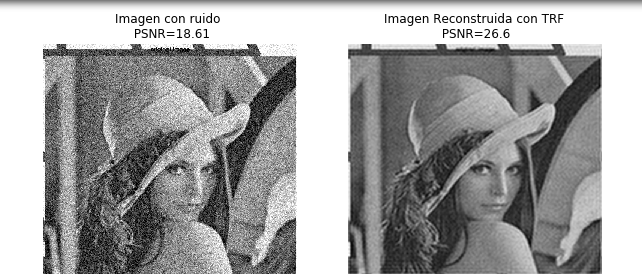
\includegraphics[width=8cm, height=4cm]{imagenes/Foto_4}
	\end{center}
	\caption{ Eliminaci\'{o}n de Ruido utilizando Transformada de Fourier en imagen de Lena\label{fig:fot_3}}%
	\end{figure}
		
	\begin{figure}[htb]%
	\begin{center}
	\includegraphics[width=8cm, height=5cm]{imagenes/Foto_5}
	\end{center}
	\caption{ Eliminaci\'{o}n de Ruido utilizando Transformada de Wavelet en imagen de Lena\label{fig:fot_4}}%
	\end{figure}
%-----------------------------------------------------------------------------------
	
%-----------------------------------------------------------------------------------
\section{Resultados}\label{sec:result}
 Para cumplir el objetivo de este proyecto se propone la implementación de dos algoritmos para la eliminación de ruido gaussiano en imágenes digitales, utilizando en uno la Transformada Discreta de Fourier y en otro Transformada Discreta de Wavelet. Ambos algoritmos parten de una imagen a la cual se le introduce ruido, en el primer algoritmo la imagen ya con ruido pasa un proceso de transformación por Fourier, luego pasa por la función filtro y reconstruimos la imagen con la inversa de Fourier, el filtro utilizado es el pasa-bandas, para el cálculo de la transformada e inversan se utiliza la librería spyci. El segundo algoritmo a partir de la imagen con ruido calcula la presencia del mismo en ella para esto se utiliza la librería de python skimage, que utiliza un filtrado por umbralización de la misma biblioteca, el cual pretende remover cualquier ruido presente y conservar la señal sin que influyan las bandas donde esta se encuentre. Para alcanzar tal fin, el filtrado por umbral desarrolla los siguientes pasos:\begin{enumerate}
\item TW a la señal,
\item Proceso de umbralización, y 
\item Transformada wavelet inversa  
\end{enumerate}

 De manera más precisa, un sistema que desarrolle los anteriores tres pasos debe asumir, en primera instancia, que los datos observados están dados bajo el modelo de señal expuesto en (3); donde $X(t)$ es la señal observada, compuesta de la señal real $S(t)$ y ruido blanco aditivo $N(t)$.

 El filtrado por umbralización pretende “limpiar” la señal $X(t)$ y recuperar una señal  $\hat{S}(t)$ como un estimativo de $S(t)$. El modelo planteado que permite esto, a través de TW, se presenta a continuación. Donde $D(.,\lambda)$ denota el operador de filtrado por umbralización con umbral $\lambda$ , y $W_{\psi,j}(.)$ y $W_{\psi,j}^{-1}(.)$, denotan la TW y su inversa respectivamente, con función wavelet $\psi$ y $j$ niveles de descomposición. \\\\
$Y = W_{\psi,j}(X)$\\\\
$Z = D(Y,\psi)$\\\\
$\hat{S}= W_{\psi,j}^{-1}(Z)$\\

 El punto clave de los métodos de eliminación de ruido que usan wavelets es que, al hacer la descomposición wavelet de una señal, esta se divide en una parte suavizada (la dada por el pasa-bajas o función de escala) y en partes que contienen los detalles de la imagen (como son los bordes). Si los detalles son pequeños (en magnitud), no cambiará sustancialmente la imagen si son eliminados. Entonces se proponen métodos de umbralizado y contracción de los coeficientes wavelet que eliminan los detalles pequeños, considerados ruido.
 
 El proceso de umbralizado se puede dividir en dos pasos:
\begin{itemize}
\item Selección del umbral $\lambda > 0$. Esta selección indica cuales coeficientes van a ser considerados como ruido y por lo tanto se van a eliminar. Un valor muy pequeño de $\lambda$ va a eliminar poco ruido y un valor muy grande va a eliminar detalles de la imagen importantes.
\item Seleccionar la función de umbralizado. Esta función debe elegirse, principalmente, de manera que se reduzca la aparición de oscilaciones alrededor de los bordes dentro de la imagen al hacer la inversión de la transformación wavelet.
\end{itemize}

 La función de umbralizado se aplica uno a uno a la magnitud de los coeficientes de $Y$ en cada banda $B^*$ de manera que
dado un coeficiente $\theta^*$ se obtiene un nuevo valor
$\hat{\theta}$:\\\\ 
$\hat{\theta} = D_t(\theta^*)$
donde $D_t(\theta^*)$ es la función de umbralizado antes mencionada. Luego de haber aplicado dicho proceso a todos los coeficientes de las bandas de $Y$ se le aplica la inversa al conjunto formado por los coeficientes obtenidos y el pasa-bajas.
Los métodos se centran principalmente en la elección del valor del umbral, tomando una de las opciones más usadas para la función de umbralizado, las llamadas funciones de ”umbralizado fuerte” y ”umbralizado suave. En el umbralizado fuerte se hace 0 a todos los coeficientes cuya magnitud sea menor que cierto umbral, sin modificar los demás coeficientes. En el caso del umbralizado suave, además de hacer 0 los coeficientes cuya magnitud sea menor que cierto valor, reduce los demás coeficientes.
En la solución utilizaremos umbralizado suave. 

 Los métodos utilizados para la selección del valor umbral en la solución propuestas son: VisuShrink y BayesShrink.
 
 El método VisuShrink consiste en aplicar umbralizado suave con valor de umbral $tuniv = \sqrt{2\log(n)} \sigma_n$, que es conocido como el umbral universal, donde $\sigma_n$  es la desviación estándar del ruido.

 El método VisuShrink sólo considera las características del ruido y no de la señal para determinar el valor del umbral. Suele sobresuavizar la imagen, ya que elimina muchos coeficientes asociados a la señal, al tratar de que todos los coeficientes asociados al ruido se anulen.
 
 En el método BayesShrink se propone un umbral adaptable a las bandas, que toma en cuenta las características de la señal presente en dichas bandas (bajo un modelo). El umbral es obtenido bajo un esquema bayesiano, asumiendo la distribución Gaussiana generalizada (GG) como distribución a priori para los coeficientes wavelet.
 
 El valor de umbral $t_B$ propuesto por el método tiene una fórmula cerrada para cada banda:
$$t_B =\frac{\sigma_n^2}{\sigma_X}$$
 
 Para estimar los parámetros, para $\sigma_n$ se usa el estimador MAD, y para $\sigma_X$ se usa el hecho de que el modelo de observación es $ Y = X + V$ (coeficientes wavelet), con $X$ y $V$ independientes, así:
$$\sigma_Y^2 = \sigma_X^2 + \sigma_V^2$$ 
y entonces se toma como estimador
$$\sigma_X^*= \sqrt{max(\sigma_Y^2 -\sigma_n^2,0 )}$$

 En la solución propuesta se utiliza la librería de python skimage y su método tal que recoge todo el proceso antes mencionado.
Mediante los resultados visuales obtenidos sobre dichas soluciones computacionales, obtenemos que con la utilización del método BayesShrink  se elimina más cantidad de ruido, luego sigue Fourier y por último VisuShrink. En resultados cuantitativos(métricas) utilizamos PSNR la cual es la relación señal/ruido pico, esta métrica se calcula mediante su relación con otra métrica la cual es MSE la cual es el error cuadrático medio.
 
 La fórmula de obtención de la $PSNR= 10 \log_{10}\left( \frac{max(k)^2}{MSE}\right)$        
donde $max(K)$ es el valor máximo que pueden llegar a tomar los píxeles de la imagen K (255) en una imagen de 8 bits por pixel. Mientras menor sea el valor del MSE, mayor lo será el del PSNR y cuando dos imágenes son idénticas, el MSE será cero y PSNR infinito. Como se muestran en la figura \ref{fig:fot_3} y \ref{fig:fot_4} según los PSNR para la primera imagen de ejemplo se obtienen los mismos resultados que los visuales y lo mismo pasa para el segundo ejemplo mostrado en el código. En complejidad algorítmica los métodos que implementan wavelet son mas rápidos que los que implementan Fourier ya que el proceso de umbralización por banda es $O(N)$, mientras que Fourier es $O(n\log(n))$.    
 
%===================================================================================
% Conclusiones
%-----------------------------------------------------------------------------------
\section{Conclusiones}\label{sec:conc}
 En la práctica, un ruido puede ser la combinación de varias componentes provenientes de fuentes y causas distintas, de modo que la reducción o atenuación puede ser desigual o limitarse a ciertas componentes del mismo. En otras palabras, debe entenderse que, debido a varios factores, el ruido no puede ser completamente eliminado de una imagen, sino sólo puede ser atenuado. La elección del filtro de atenuación dependerá del factor que se busque dentro de la imagen y si se está dispuesto a sacrificar calidad o bordes de la imagen. O bien, si esto no es el resultado final esperado, deberán aplicarse más técnicas de procesamiento e ir adaptándolas con los medios adecuados para perder la menor cantidad de información posible. 
  
 La Transformada de Fourier es ampliamente utilizada en el procesamiento y análisis de señales y con resultados satisfactorios en los casos en que estas señales son periódicas y lo suficientemente regulares, pero no ocurre lo mismo para el análisis de señales cuyo espectro varía con el tiempo. La Transformada de Fourier detecta la presencia de una determinada frecuencia pero no brinda información acerca de la evolución en el tiempo de las características espectrales de la señal. Muchos aspectos temporales de la señal, tales como el comienzo y el fin de una señal finita y el instante de aparición de una singularidad en una señal transitoria, no pueden ser analizados adecuadamente por el análisis de Fourier. 
 
 Una herramienta matemática que permite resolver estos problemas es la Transformada Wavelet. Este tipo de transformada es capaz de concentrarse en fenómenos transitorios y de alta frecuencia. El punto clave de los métodos de eliminación de ruido que usan wavelets es que, al hacer la descomposición wavelet de una señal, esta se divide en una parte suavizada (la dada por el pasa-bajas o función de escala) y en partes que contienen los detalles de la imagen (como son los bordes). Si los detalles son pequeños (en magnitud), no cambiara sustancialmente la imagen si son eliminados. Entonces se proponen métodos de umbralizado y contracción de los coeficientes wavelet que eliminan los detalles pequeños, considerados ruido. En la literatura existen varios métodos de elección del valor de umbral, en este trabajo nos enfocamos en: BayesShrink y VisuShrink. Otro punto a favor del uso de la Transformada Wavelet es su complejidad algorítmica ya que es de O(n), mientras q la Transformada Rapida de Fourier es de orden O(nlogn).  
   
%===================================================================================

%===================================================================================
% Recomendaciones
%-----------------------------------------------------------------------------------

%===================================================================================

%===================================================================================
% Bibliografía
%-----------------------------------------------------------------------------------
\begin{thebibliography}{99}
%-----------------------------------------------------------------------------------
	
	\bibitem{morel05} Morel, A. B. (2005). A review of image denoising algorithms, with a new one.

	\bibitem{egiazarian09} Egiazarian, K. D. (2009). BM3D Image Denoising with Shape-Adaptive Principal Component Analysis.

	\bibitem{tomasi98} Tomasi, C., and Manduchi, R. (1998). Bilateral filtering for gray and color images.

	\bibitem{galvez17} Galvez, Y. (2017). Suavizado de imágenes digitales mediante procesamiento a nivel de subpíxel.

	\bibitem{estrtada12} Estrada, C. D. (2012). Un filtro para la eliminación de ruido mediante correlación espacial en imágenes.

	\bibitem{perez15} Pérez, C. (2015). Diseño de filtros para el procesado de imágenes basados en teoría de grafos.
	
	\bibitem{guerrero11} Guerrero, J. A. (2011). Conjuntos Completos de Filtros Para la Eliminación de Ruido en Imágenes.

%-----------------------------------------------------------------------------------
\end{thebibliography}
%-----------------------------------------------------------------------------------

\label{end}

\end{document}

%===================================================================================